\section{Auswertung}

\subsection{Dokumentation zur Analyse der Umfragebögen}

Jede Frage im Umfragebogen wurde kategorisiert. Dabei ergaben sich drei Arten: 

Die erste Art waren Fragen, die dazu dienten, die Ergebnisse der befragten Person zu Klassifizieren, um so am Ende Unterschiede und Zusammenhänge zwischen einzelnen Gruppen entdecken zu können. Dazu zählten die Fragen zum Geschlecht und zum Alter. 

Bei der zweiten Art handelte es sich um Fragen, die die Umfrageteilnehmer selbständig mit individuellen Zahlen ausfüllen sollten. Die hierbei eingegebenen Werte wurden paraphrasiert dokumentiert. 

Zum Schluss handelt es sich um ein Multiple Choice Verfahren, indem die Antwortmöglichkeiten vorgegeben waren und der Befragte nur zutreffendes ankreuzen musste. Jedem möglichen Feld wurde eine Zahl zwischen 0 und 10 zugewiesen. Es wurden alle angekreuzten Felder im Record Data dokumentiert.

Die nun folgenden Beispiele sollen dieses veranschaulichen. Sie sind universell gültig, auf ein minimum Reduziert und können auch zum Auswerten anderer Umfragen verwendet werden. Dabei ist NumberHolder ein Record, welches eine reelle Zahl abspeichern kann und QuestionHolder eine Klasse, die ein Array zurückgibt, welches die Nummern der Felder aller ausgewählten Fragen beinhaltet. Alle Fragen wurden nach dem Alter sortiert ausgewertet. Für die Ergebnisse wurden zwei Algorithmen geschrieben, eines für die Fragen mit individuellen Antworten und eines für Multiple Choice Fragen. Um auf ein vergleichbares Ergebnis trotz schwankender Teilnehmeranzahl pro Altersstufe zu kommen, wird alles in Prozent berechnet. Jeder Algorithmus besteht aus zwei Listen, einer beinhaltet die totalen Werte und eine die Anzahl an Personen pro Teilnehmer. Die Division ergibt das prozentuale Ergebnis für jede Altersgruppe.

Um mit den Algorithmen eine möglichst modulare Struktur zu haben, die sich auf eine Veränderung der Analyse der Fragen anpasst, verwende ich Interfaces, welche eine sehr hohe Flexibilität über Lambda-Ausdrücke erreicht.

\subsection{Datenwerte}

Insgesamt wurden 160 Personen am FGB befragt. Von diesen 160 Personen fallen 133 Personen in die zu betrachtende Zielgruppe. Innerhalb dieser 33 Personen sind 67 Personen männlich, 58 Personen weiblich und 8 divers.

Der Altersduchschnitt aller Befragten liegt bei 15,02 Jahren und innerhalb der Zielgruppe bei 15,34 Jahren. Da das minimale und das maximale Alter bei jeweils 13 und 18 Jahren liegt, umfasst die Spannweite 6 Jahre und der Median beträgt 15,5 Jahren. Damit liegt der Altersdurchschnitt etwas unter dem Median. Dadurch ist das Alter innerhalb der Befragten etwas jünger. 

Die Gesamtteilnehmer nutzen das Internet im Durchschnitt erstmals im Alter von 7,63 Jahren. Bei meiner Zielgruppe liegt die Erstnutzung im Alter von 7,68 Jahren. Am Frühesten nutzen Teilnehmer dieses mit 4 Jahren, spätestens mit 12. Der Median und die Spannweite liegen somit bei 8 Jahren.

In der zweiten Frage liegt die durchschnittliche Nutzung des Internets pro Tag bei allen Befragten bei 4,77 Stunden und innerhalb der Zielgruppe bei 5 Stunden. Minimal wurde das Internet 0 Stunden genutzt, maximal 12 Stunden. Der Median liegt damit bei 6 und die Spannweite bei 12 Stunden am Tag.

Bei der Frage nach der Regelmäßigkeit gaben von den insgesamt 133 Personen 55 von sich aus an, dass sie das Internet mehr als zwei bis dreimal am Tag nutzen. Nur ein Teilnehmer kreuzte an, dass er das Internet seltener als täglich nutzen würde. Niemand gab an, dass er seltener als 2 bis 3 mal im Monat das Internet nutzt.

Innerhalb der Befragten war das Handy das mit Abstand beliebteste Gerät zur Nutzung des Internets. Von den insgesamt 133 nutzten 125 das Handy. Auf Platz zwei lag der Laptop mit 87 Personen. Die am seltensten genutzten Geräte waren jene, die unter Sonstiges fallen. Dieses Feld wurde von nur 12 Personen angekreuzt.

\begin{figure}[ht]
    \centering
    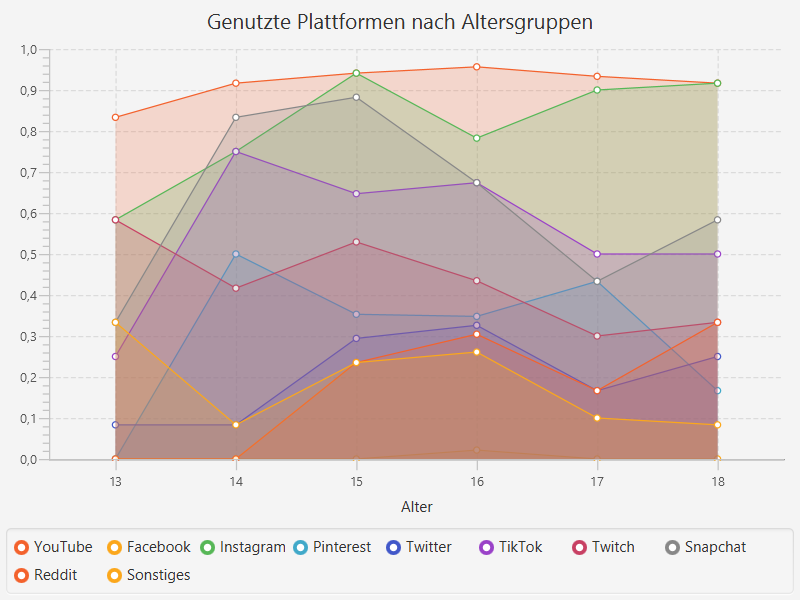
\includegraphics[width=8.5cm]{image/Diagramm Genutzte Plattformen.png}
    \caption{\label{imgs:diagramm_plattformen_datenwerte}Nutzung Social Media basierter Plattformen}
\end{figure}

Als die Umfrageteilnehmer die genutzten Plattformen ankreuzen sollten, lagen YouTube, Instagram, Snapchat und TikTok mit jeweils 120, 106, 80 und 75 Kreuzen sehr weit vorne. Sowohl bei der Plattform Pintrest, als auch Reddit konnte ein großer Unterschied zwischen Mädchen und Jungen festgestellt werden. Während Pinterest 72,09 \% Frauen nutzen, sind bei Reddit 77,77 \% männliche Nutzer. Facebook lag auf dem letzten Platz mit einem einzigen Nutzer.

\begin{figure}[ht]
    \centering
    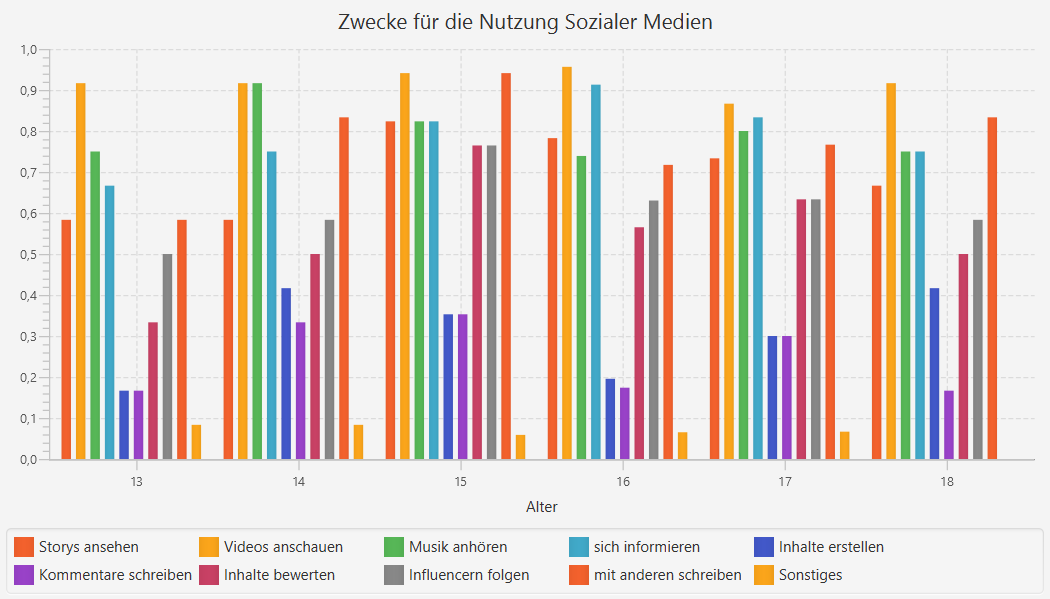
\includegraphics[width=10cm]{image/Diagramm Zwecke der Nutzung.png}
    \caption{\label{imgs:diagramm_zwecke_datenwerte}Zwecke zur Nutzung von sozialen Medien}
\end{figure}

Als Grund für eine Nutzung von sozialen Medien geben 119 Personen an, dass sie unterhalten werden wollen. Es gaben 105 Personen an, dass sie sich dort informieren sowie mit Anderen schreiben möchten.

Die Meisten der Befragten nutzen soziale Medien zum Anschauen von Videos (119 Personen), zum Informieren (107 Personen) sowie zum Hören von Musik (101 Personen). Besonders selten nutzen die Umfrageteilnehmer soziale Medien zum Erstellen eigener Inhalte sowie zum Kommentieren von Inhalten.

In der Frage nach den Gründen sowie nach der Nutzung von sozialen Medien ist das Verhältnis zwischen männlichen und weiblichen Befragten bei jedem Feld nahezu identisch. Das Verhältnis von Personen mit einer diversen Geschlechteridentität wird bewusst weggelassen, da diese mit einer Gesamtanzahl von 8 Personen zu niedrig ist, um eine sinnvolle und zielgerichtete Analyse durchzuführen.

\subsection{Regelmäßigkeiten}

\begin{figure}[h]
    \centering
    \includegraphics[width=8.5cm]{image/Diagramm Geräte.png}
    \caption{\label{imgs:diagramm_geraete_regelmaesigkeit}Nutzung von Geräten}
\end{figure}

Das Nutzen von Handys ist durchgängig unabhängig vom Alter auf einem hohen Wert. Dies hängt wahrscheinlich damit zusammen, dass sie im Vergleich mit anderen Geräten, wie zum Beispiel einem PC, wesentlich günstiger sind sowie den Bonus haben, Verfügbarkeit und Leistung zu kombinieren.

Einige Plattformen, die zurzeit in der Mode sind, wurden durchgängig unabhängig von der Altersgruppe häufig angekreuzt. Dies war ein zu erwartendes Ergebnis, welches lediglich die von den jeweiligen  Plattformen veröffentlichten Nutzerstatistiken bestätigen. Die einzige Schlussfolgerung daraus ist, dass Jugendliche am FGB im Durchschnitt die selben sozialen Plattformen nutzen wie andere Jugendliche auf der ganzen Welt.

Die Plattform YouTube ist die einzige, von den vorgegebenen Plattformen, auf der die Nutzer sich informieren, unterhalten und mit anderen schreiben können. Dadurch ergibt sich eine hohe Nutzung, die sehr regelmäßig in allen Altersgruppen ist.

\subsection{Anomalien}

\begin{figure}[h]
    \centering
    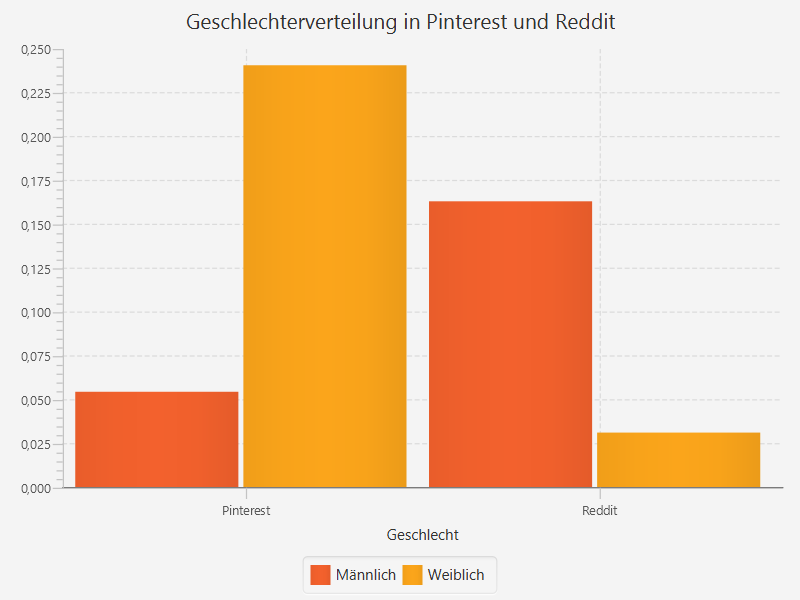
\includegraphics[width=8.5cm]{image/Diagramm Pinterst vs Reddit.png}
    \caption{\label{imgs:diagramm_pinterest_reddit}Geschlechterverteilung bei Pinterest und Reddit}
\end{figure}

Die größte Anomalie bezüglich der Geschlechterverteilung tritt in der Nutzung von Pinterest und Reddit auf. Diese Anomalie konnte nicht mit dem Wissen, welches aus anderen Fragen gewonnen wurde, erklärt werden. Ich vermute, dass die angebotenen Inhalte der Plattformen diese Diskrepanz hervorrufen. Da allerdings in der Umfrage nicht nach so etwas gefragt wurde, ist es mir nicht möglich, diese These zu belegen.Es lässt sich statistisch erkennen, dass die 17-Jährigen die untersuchten Plattformen weniger nutzen. Dieses könnte damit zusammenhängen, dass diese Altersgruppe sich intensiv auf das Abitur vorbereitet und dadurch weniger Zeit für die Nutzung sozialer Medien verwendet.

\subsection{Fehlerbetrachtung}

Die dritte Frage: \glqq Seit wann (Jahr, ungefähr) nutzt du das Internet?\grqq \nobreakspace war ungenau. Diese Frage hätte ich besser präzisieren müssen, da im Ergebnis der Befragung ein großer Interpretationsspielraum entstand. Viele Umfrageteilnehmer füllten diese Frage falsch aus, so dass für die Datenbank die Ergebnisse geändert werden mussten. Am Ende musste die Matrix, bestehend aus $JJJJ$, mit dem Ergebnis übereinstimmen. Beim Paraphrasieren können Fehler
auftreten, wodurch dieser Wert falsch verstanden und somit auch verfälscht eingetragenen wurde.

Die Spannweite vieler Fragen ist vom Median meist sehr weit entfernt. Extremwerte, die hierbei auftreten, hätten allerdings durch die Masse der befragten Personen ausgeglichen werden sollen. Da ich aber nur 133 Personen, die auch in meiner Zielgruppe fallen, befragt habe, sind die Mittelwerte der Ergebnisse verfälscht.

Für eine möglichst kleine Fehlerspanne wären daher 500 Befragte\cite{aussagekraft} notwendig gewesen. Da ich zurzeit aber weniger Umfrageteilnehmer habe, rechne ich mit einer Fehlerspanne von etwa 5 \%.